\documentclass[11pt, oneside]{article} 
\usepackage{geometry}
\geometry{letterpaper} 
\usepackage{graphicx}
	
\usepackage{amssymb}
\usepackage{amsmath}
\usepackage{parskip}
\usepackage{color}
\usepackage{hyperref}

\graphicspath{{/Users/telliott_admin/Tex/png/}}
% \begin{center} 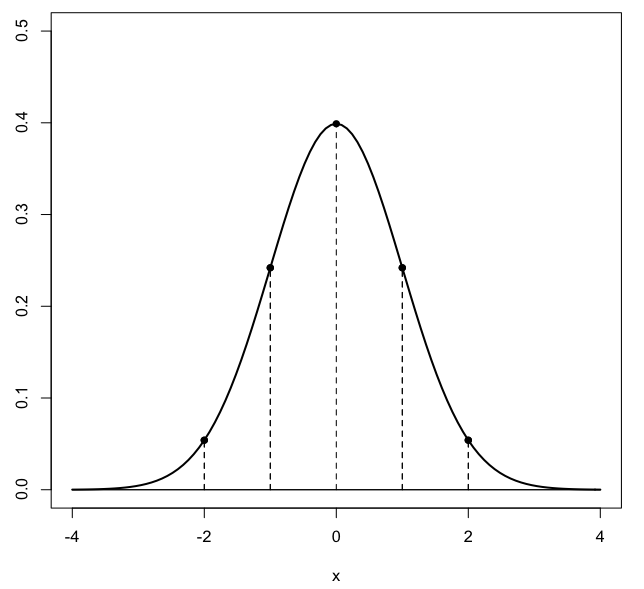
\includegraphics [scale=0.4] {gauss3.png} \end{center}

\title{Introduction}
\date{}

\begin{document}
\maketitle
\Large

\subsection*{Curvature of curves}
We would like to have a way to describe the curvature of a curve at a point.  The way this is done is to fit a circle to the curve, to construct a circle that has the same first and second derivatives as the curve at the point of interest.  (This section is taken from Hamming).

The general equation of a circle is
\[ (x-h)^2 + (y-k)^2 = r^2 \]

Implicit differentiation gives
\[ 2(x - h) + 2(y - k) \ y' = 0 \]
\[ (x - h) + (y - k) \ y' = 0 \]

Differentiate again (using the product rule)
\[ 1 + (y')^2 +  (y - k) \ y''  = 0 \]

The known values in these equations are the point $(x,y)$, the slope $y'$ and the second derivative $y''$, taken from the curve we want to analyze.  

The unknowns are the parameters of the circle that we're trying to find:  $h,k,$ and $r$.  

Now, solve the last equation for 
\[ y - k = - \frac{1 + (y')^2}{y''} \]

and solve the second equation for
\[ x - h = -(y - k)\ y' \]

From these two equations we can find $h$ and $k$, the center of the circle.

Substituting for $x-h$ into the general equation of the circle we obtain

\[ (y - k)^2 \ (y')^2 + (y-k)^2 = r^2 \]
\[ (y-k)^2 \ [ \ (y')^2 + 1 \ ]  = r^2 \]

Now substitute for $y-k$

\[ [ \ \frac{1 + (y')^2}{y''} ]^2 \  [ \ (y')^2 + 1 \ ] = r^2 \]
\[ \frac{\ [ \ 1 + (y')^2 \ ]^3}{(y'')^2} = r^2 \]

Take the square root to find the radius.

\[  r =  \frac{\ [ \ 1 + (y')^2 \ ]^{3/2}}{y''} \]

If the original curve had been a straight line or the second derivative zero at that point, we would face the problem of dividision by zero.  

For this reason, it makes sense to define the \emph{curvature} as the inverse of the radius of the fitted circle.  $\kappa$ is used for the curvature:

\[ \kappa = \frac{1}{r} = \frac{y''}{[ \ 1 + (y')^2 \ ]^{3/2}} \]

We write this as the absolute value:
\[ \kappa = \frac{1}{r} = | \frac{y''}{[ \ 1 + (y')^2 \ ]^{3/2}} | \]

because $r$ is always a positive quantity.

So, for example, any straight line (which has $y'' = 0$), has zero curvature.

\subsection*{test with a known circle}
Try using a circle centered at $(0,0)$, as the curve to be fitted.  We should get back $h=0, k=0, r=r$.

\[ x^2 + y^2 = r^2 \]
\[ 2x + 2y \ y' = 0 \]
\[ y' = -\frac{x}{y} \]

The second derivative is
\[ y'' = - \ [ \frac{y - y' x}{y^2} \ ] \ \]

Combined with the previous result
\[ y'' = - \ [ \frac{y - (-x/y) \cdot x}{y^2} \ ] \ \]
\[ = - \frac{y^2 + x^2}{y^3} = - \frac{r^2}{y^3} \]

Calculate the three values:

\[ \kappa = | \frac{y''}{[ \ 1 + (y')^2 \ ]^{3/2}} | \]
\[ = \frac{r^2}{y^3} \cdot \frac{1}{(1 + x^2/y^2)^{3/2}} \]
\[ = r^2 \cdot \frac{1}{[ \ y^2(1 + x^2/y^2) \ ]^{3/2}} \]
\[ = r^2 \cdot \frac{1}{[ r^2\ ]^{3/2}} \]
\[ = \frac{1}{r} \]

That's exactly what we want.  $\kappa = 1/r$ corresponds to a circle of radius $r$.  To find the center of the circle:
\[ y - k = - \frac{1 + (y')^2}{y''} \]
\[ = \frac{1 + x^2/y^2}{r^2/y^3} \]
\[ = \frac{y^2 + x^2}{r^2/y} \]
\[ = y \]

For $x$
\[ x - h = -(y - k)\ y' \]
\[ = -(y - k) (-\frac{x}{y}) \]
Since we found that $k = 0$
\[ x - h = -y(-\frac{x}{y}) = x \]

Everything looks correct.  Having carried out all of this preparation, let's do a real problem.

\subsection*{parabola}

Consider a simple parabola
\[ y = x^2 \ \ \ \ y' = 2x \ \ \ \  y'' = 2 \]

The radius is
\[  r =  | \frac{\ [ \ 1 + (y')^2 \ ]^{3/2}}{y''} | \]
\[ =  \frac{\ [ \ 1 + 4x^2 \ ]^{3/2}}{2} \]

The $y$-coordinate of the origin of the circle, $k$, is
\[ k = y + \frac{1 + (y')^2}{y''} \]
\[ = y + \frac{1 + 4x^2}{2} \]
and $h$ is
\[ h =  x + (y - k)\ 2x \]

If we decide to fit the circle to the parabola at the point $(0,0)$ we have
\[ r = \frac{1}{2}  \ \ \ \  k = \frac{1}{2}  \ \ \ \  h = 0 \]

Perhaps more interesting, for the point $(1,1)$ we have
\[ r = \frac{5^{3/2}}{2} \]

\[ k = y + \frac{1 + 4x^2}{2} \]
\[ = 1 + \frac{5}{2} = \frac{7}{2} \]

\[ h =  x + (y - k)\ 2x \]
\[ = 1 + (1 - 7/2) 2 = -4  \]

Which seems to be correct.
\begin{center} 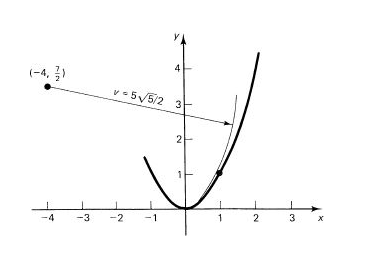
\includegraphics [scale=0.75] {curvature.png} \end{center}
Find the slope of the line from the center of the circle to $(1,1)$:
\[ m = \frac{1 - k}{1 - h} \]
\[ = \frac{1 - 7/2}{1 -  (-4)} = \frac{-5/2}{5} = - \frac{1}{2} \]
Recall that slope of the parabola at $(1,1)$ is $y' = 2x = 2$.  The slope of the line perpendicular to the tangent to the curve at the point $(1,1)$ is the negative of the reciprocal, which is just what we obtained.

The squared distance between the center and the point should be equal to the radius squared from above:
\[ (1 - 7/2)^2 + (1 - (-4))^2 \]
\[ = \frac{1}{4} \cdot 5^2 + 5^2 = \frac{5}{4} \cdot 5^2 = \frac{5^3}{4} \]
Taking the square root, we obtain what we had above:
\[ r = \frac{5^{3/2}}{2} \]

Notice that the point $(1,1)$ is $5$ units horizontally across from the center and $5/2$ units down.  If we were to translate the whole thing to the origin and then find the slope of the tangent to the circle at that point it would be
\[ -\frac{x}{y} = - \frac{5}{5/2} = - 2 \]
which is the same as the slope of the parabola at that point, within sign.

The second derivative is
\[ y'' =  - \frac{r^2}{y^3} \]
\[ = - \frac{5^3/4}{(5/2)^3} = -2  \]
which is also the same, within sign.  The difference in sign comes about because we have not adjusted the equation for the circle.  This point is in the fourth quadrant for the version moved to the origin.

\end{document}